% ID: SEL-D0015-BB-E04
% ESTADO: validada. S016. Revisión matemática, didáctica y visual.
\textbf{a) Producto, cadena y cociente.}\par\nopagebreak[4]
Para la primera función,
\[
\begin{aligned}
f'(x)&=4x(x^2-5)e^{3x}+3(x^2-5)^2e^{3x}\\
&=\boxed{(x^2-5)e^{3x}(3x^2+4x-15).}
\end{aligned}
\]
Está definida en todo $\mathbb R$. Para la segunda ponemos $Q=x^3-5x$, de modo que $(\ln Q)'=(3x^2-5)/Q$. Aplicando el cociente,
\[
\boxed{g'(x)=\frac{\dfrac{3x^2-5}{x^3-5x}(1-x^2)+2x\ln(x^3-5x)}{(1-x^2)^2}.}
\]
El dominio real exige $x^3-5x>0$ y $x\ne\pm1$. Al estudiar el signo de $x(x^2-5)$ se obtiene
\[
\boxed{(-\sqrt5,-1)\ \cup\ (-1,0)\ \cup\ (\sqrt5,+\infty).}
\]
El signo positivo del término $2x\ln Q$ procede de restar el producto por la derivada del denominador, que es $-2x$.

\textbf{b) Área acotada con el eje.}\par\nopagebreak[4]
Los cortes satisfacen $-x^2+2x+3=0$, es decir, $(x-3)(x+1)=0$: $x=-1$ y $x=3$. La parábola $h=4-(x-1)^2$ es no negativa entre esas raíces.
\begin{center}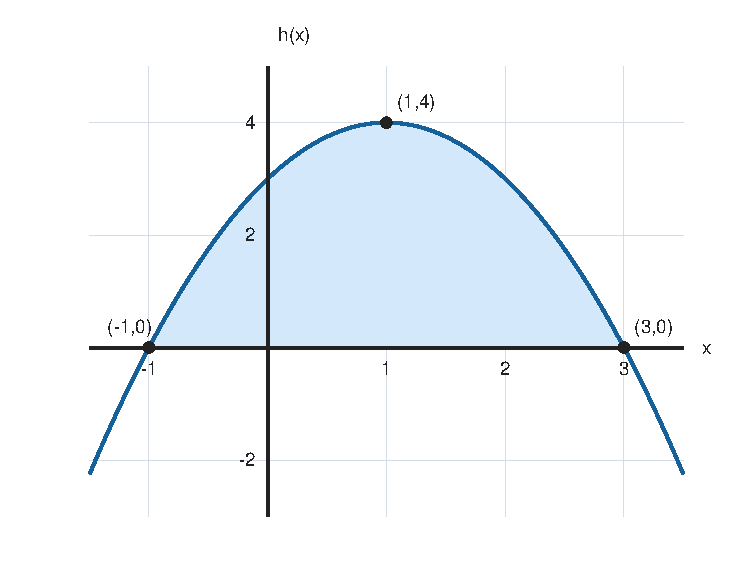
\includegraphics[width=0.56\linewidth]{recursos/figuras/s016-area.pdf}\end{center}
\[
\begin{aligned}
\mathcal A&=\int_{-1}^{3}(-x^2+2x+3)\,dx\\
&=\left[-\frac{x^3}{3}+x^2+3x\right]_{-1}^{3}
=9-\left(-\frac53\right)
=\boxed{\frac{32}{3}\text{ unidades cuadradas}.}
\end{aligned}
\]
La simetría respecto a $x=1$ permite contrastarlo con $\int_{-2}^2(4-u^2)\,du=32/3$.
